% !TEX root = ./Vorlesungsmitschrift AGLA 2.tex  
\lecture{Di 12.05. 10:15}{}
\begin{idee*}
  Sei
  \begin{align*}
    P(x_1,\dotsc,x_n)=\sum\limits_{1\leq i\leq j\leq n}\alpha_{ij}x_i x_j+\sum\limits_{1\leq i \leq n}\alpha_{0i}x_i\cdot 1+\alpha_{00}\cdot 1^2.
  \end{align*}
  Wir schreiben
  \begin{align*}
    x'=\begin{pNiceMatrix} 1\\ x_1 \\ \vdots \\ x_n \end{pNiceMatrix}\in K^{n+1}.
  \end{align*}
  und (sei im Folgenden \( \characteristic K\neq 2 \))
  \begin{align*}
    A=\begin{pNiceArray}{C|CCCC}
      a_{00}& a_{01} & \Cdots & \Cdots & a_{0n} \\
      \hline
      a_{10} & a_{11} & a_{12} & \Cdots & a_{1n} \\
       \Vdots & \Vdots & \Ddots &  & \Vdots \\
       \\
       a_{n0} & a_{n1} & \Cdots & \Cdots & a_{nn}
    \end{pNiceArray}
  \end{align*}
  mit \( a_{ii}=\alpha_{ii}\quad \forall 0\leq i\leq n \).
  \begin{align*}
    a_{ij}=a_{ji}=\frac{1}{2}\alpha_{ij}\text{ für }0\leq i<j\leq n.
  \end{align*}
  Es gilt dann
  \begin{align*}
    P(x_1,\dotsc,x_n)=\transpose{x'}A'x'
  \end{align*}
  und
  \begin{equation*}
    Q=\Set{(x_1,\dotsc,x_n)\in K^n| \transpose{x'}A'x'=0}.
  \end{equation*}
\end{idee*}
\begin{bemerkung*}
  Die Matrix \( A' \) ist symmetrisch (nach Konstruktion).
\end{bemerkung*}
\begin{definition*}
  In obiger Notation nennen wir \( A' \) di erweiterte Matrix zu \( P \) und \( x' \) den erweiterten Spaltenvektor zu \( x \). Wir sagen, dass \( A'\in \matrices{(n+1)}{(n+1)}{K} \) die Quadrik \( Q \) beschreibt, wenn gilt
  \begin{equation*}
    Q=\Set{x\in K^n|\transpose{x'}A'x'=0}.
  \end{equation*}
\end{definition*}
\begin{notation*}
  Für \( P \) wie oben schreiben wir
  \begin{equation*}
    A=\begin{pNiceMatrix}
      a_{11} & \Cdots & a_{1n} \\
      \Vdots &  & \Vdots \\
      a_{n1} & \Cdots & a_{nn}
    \end{pNiceMatrix}
  \end{equation*}
  für den \enquote{rein quadratischen} Anteil von \( P \).
\end{notation*}
\begin{bemerkung*}
  Sei \( Q\subseteq K^n \) eine Quadrik. Dann gibt es im Allgemeinen nicht nur eine erweiterte Matrix \( A' \) die \( Q \) beschreibt. Ist
  \begin{equation*}
    Q=\Set{(x_1,\dotsc,x_n)\in K^n| \transpose{x'}A'x'=0},
  \end{equation*}
  dann beschreibt auch \( \lambda A' \) mit \( \lambda\in K\setminus\zeroset \) die Quadrik \( Q \).
\end{bemerkung*}
\begin{frage*}
  Wie verhalten sich Quadriken unter Koordinatentransformationen / Affinitäten?
\end{frage*}
\begin{beispiel*}
  \( K=\rationals \). \( P(x_1,x_2)=x_1^2+x_2^2 \).
  \begin{align*}
    \begin{pNiceMatrix} x_1 \\ x_2 \end{pNiceMatrix}&\begin{aligned}[t]
      &=\begin{pNiceMatrix} y_1+y_2 \\ y_2+1 \end{pNiceMatrix}\\
      &=\begin{pNiceMatrix} 1 & 1 \\ 0 & 1 \end{pNiceMatrix}\begin{pNiceMatrix} y_1 \\ y_2 \end{pNiceMatrix}+\begin{pNiceMatrix} 0 \\ 1 \end{pNiceMatrix}.
    \end{aligned}\\
    P(x_1,x_2)&\begin{aligned}[t]
      &=(y_1+y_2)^2+(y_2+1)^2\\
      &=y_1^2+2y_1 y_2+2 y_2^2+2y_2+1
    \end{aligned}
  \end{align*}
  ist wieder ein quadratisches Polynom.
\end{beispiel*}
\begin{lemma}\label{affinitaet_bildet_quadriken_auf_quadriken_ab}
  Sei \( K \) ein Körper mit \( \characteristic K\neq2 \), \( Q\leq K^n \) eine Quadrik und \( f\maps K^n\to K^n \) eine Affinität. Dann ist auch \( f(Q)\subseteq K^n \) eine Quadrik.
\end{lemma}
\begin{proof}
  Sei \( Q \) gegeben durch das quadratische Polynom \( P(x_1,\dotsc, x_n) \), also
  \begin{equation*}
    Q=\Set{(x_1,\dotsc,x_n)\in K^n|P(x_1,\dotsc,x_n)=0}.
  \end{equation*}
  Sei \( A' \) die erweiterte Matrix zu \( P \) und \( x' \) der erweiterte Spaltenvektor zu \( x \). Dann gilt
  \begin{align*}
    Q=\Set{(x_1,\dotsc,x_n\in K^n)|\transpose{x'}A'x'=0}.
  \end{align*}
  Als nächstes beschreibe den durch \( f \) gegebenen Koordinatenwechsel. \( f \) ist eine Affinität, also \texists \( b\in K^n \) und \( S\in \invertiblematrices{n}{K} \) mit
  \begin{equation*}
    \begin{split}
      f\maps K^n&\to K^n\\
      x&\mapsto Sx+b.
    \end{split}
  \end{equation*}
  Sei \( y=f(x) \), schreibe \( y'=\begin{pNiceMatrix} 1 \\ y_1 \\ \Vdots \\ y_n \end{pNiceMatrix} \),
  \begin{equation*}
    S'=\begin{pNiceArray}{C|CCC}
      1 & 0 & \Cdots & 0 \\\hline
      b_1 & \Block{3-3}<\LARGE>{S} &  & \\
      \Vdots & & & \\
      b_n & & &
    \end{pNiceArray}.
  \end{equation*}
  Dann gilt \( y'=S'x' \).
  \begin{bemerkung*}
    \( S' \) ist invertierbar mit inverser Matrix
    \begin{equation*}
      T'=\inv{(S')}=\begin{pNiceArray}{C|CCC}
        1 & 0 & \Cdots & 0 \\\hline
         & \Block{3-3}<\LARGE>{\inv{S}} &  & \\
         -\inv{S}b & & & \\
         & & &
      \end{pNiceArray},
    \end{equation*}
    \dh \( x'=T'y' \).
  \end{bemerkung*}
  Es gilt
  \begin{equation*}
    \begin{split}
      f(Q)&=\Set{f((x_1,\dotsc,x_n))\in K^n| P(x_1,\dotsc,x_n)=0}\\
      &=\Set{y\in K^n| \transpose{x'}A'x'=0}\\
      &=\Set{y\in K^n| \transpose{T'y'}A'(T'y')=0}\\
      &=\Set{y\in K^n| \underset{\hphantom{\text{symmetrische Matrix}}}{\transpose{y'}\underbrace{\transpose{T'}A'T'}_{\mathclap{\text{symmetrische Matrix}}}y'}=0},
    \end{split}
  \end{equation*}
  also ist \( f(Q) \) eine Quadrik mit
  \begin{equation*}
    P'(y_1,\dotsc, y_n)=\transpose{y'}(\transpose{T'}A'T')y'.
  \end{equation*}
\end{proof}
\begin{bemerkung*}
  Der Beweis von \thref{affinitaet_bildet_quadriken_auf_quadriken_ab} zeigt wie sich eine beschreibende Matrix \( A' \) unter einer Koordinatentransformation ändert.
\end{bemerkung*}
\begin{frage*}
  Sei \( Q \) eine Quadrik beschrieben durch eine erweiterte Matrix \( A' \). Find eine Koordinatentransformation \( f \) der \( K^n \), sodass \( f(Q) \) möglichst \enquote{einfach} beschrieben werden kann.
\end{frage*}
\minisec{zweiter Schritt}
Entferne lineare Terme
\begin{equation*}
  (y_1+1)^2+(y_2-1)^2-2=0.
\end{equation*}
Nach der Koordinatentransformation
\begin{equation*}
  z_1=y_1+1\qquad z_2=y_2-1
\end{equation*}
erhalten wir \( z_1^2+z_2^2=2 \), oder nach skalieren mit \( \sqrt{2} \)
\begin{gather*}
  \sqrt{2}w_1= z_1\qquad \sqrt{2}w_2=z_2\\
  w_1^2+w_2^2=1
\end{gather*}
\begin{figure}[H]
  \centering
  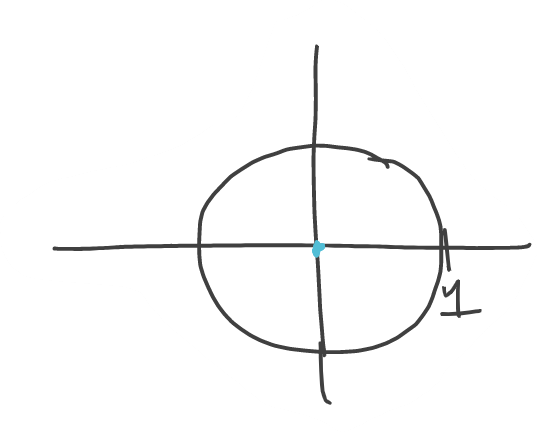
\includegraphics[width=0.5\linewidth]{figures/vereinfachte_quadrik}
  \label{fig:vereinfachte_quadrik}
\end{figure}
\begin{satz}[affine Hauptachsentransformation von reellen Quadriken]\label{affine_hauptachsentranformation_reelle_quadriken}
  Sei \( A'\in \matrices{(n+1)}{(n+1)}{\reals} \) eine symmetrische Matrix und die Quadrik \( Q\subseteq \reals^n \) gegeben durch
  \begin{equation*}
    Q=\Set{(x_1,\dotsc,x_n)\in \reals^n|\transpose{x'}A'x'=0}.
  \end{equation*}
  Sei \( A \) der rein quadratische Anteil von \( A' \), \( m=\rang A \) und \( m'=\rang A' \). Dann gibt es eine Affinität \( f\maps \reals^n\to \reals^n \), sodass \( f(Q) \) beschrieben wird durch eine der folgenden Gleichungen:
  \begin{eigenschaftenenumerate}
    \item \( m=m' \):
    \begin{equation*}
      y_1^2+\dotsb+y_k^2-y_{k+1}^2-\dotsb-y_m^2=0
    \end{equation*}
    für ein \( 0\leq j \leq m \).
    \item \( m+1=m' \):
    \begin{equation*}
      y_1^2+\dotsb+y_k^2-y_{k+1}^2-\dotsb-y_m^2=1
    \end{equation*}
    für ein \( 0\leq k \leq m \).
    \item \( m+2=m' \):
    \begin{equation*}
      y_1^2+\dotsb+y_k^2-y_{k+1}^2-\dotsb-y_m^2+2_{y_{m+1}}=0
    \end{equation*}
    für ein \( 0\leq k\leq m \).
  \end{eigenschaftenenumerate} 
\end{satz}
\begin{frageuebung}
  Warum gilt immer \( m\leq m'\leq m+2 \)?
\end{frageuebung}
\begin{proof}[Beweis zu \thref{affine_hauptachsentranformation_reelle_quadriken}]
  Sei
  \begin{equation*}
    A'=\begin{pNiceArray}{C|CCC}
      a_{00} & a_{01} & \Cdots & a_{0n} \\\hline
      a_{10} & \Block{3-3}<\LARGE>{A} &  & \\
      \Vdots & & & \\
      a_{n0} & & &
    \end{pNiceArray}.
  \end{equation*}
  mit \( A\in \matrices{n}{n}{\reals} \).
  \begin{proofenumerate}[label=Schritt \arabic*]
    \item Entferne gemischte Terme.
    \begin{idee*}
      Wollen \( A \) in Diagonalgestalt bringen. 
    \end{idee*}
    \aglacourse{1}: Orthogonalisierungssatz für reelle symmetrische Matrizen.

    Wir erhalten eine invertierbare Matrix \( T_1\in \invertiblematrices{n}{\reals} \) mit
    \begin{equation*}
        \transpose{T_1}AT_1=\begin{pNiceArray}{C|C|C}
            I_k & 0 & 0\\\hline
            0 & -I_{m-k} & 0\\\hline
            0 & 0 & 0
        \end{pNiceArray},
    \end{equation*}
    \( I_l \) Einheitsmatrix der Dimension \( l \), \( m=\rang A \), \( k \) Zahl der positiven Eigenwerte von \( A \) (mit Vielfachheit).

    Sei
    \begin{equation*}
      T_1'=\begin{pNiceArray}{C|CCC}
        1 & 0 & \Cdots & 0 \\\hline
        0 & \Block{3-3}<\LARGE>{T_1} &  & \\
        \Vdots & & & \\
        0 & & &
      \end{pNiceArray}.
    \end{equation*}
    Dann gilt
    \begin{equation*}
      \begin{split}
        A_1'&\definedas \transpose{T_1'}A'T_1'\\
        &=\begin{pNiceArray}{C|CCC}[create-large-nodes]
          c_{00} & c_{01} & \Cdots & c_{0n} \\\hline
          c_{10} & I_k   & 0   &0    \\\cline{2-4}
          \Vdots & 0  & -I_{m-k}   &0 \\\cline{2-4}
          c_{n0} & 0    & 0    & 0
          \CodeAfter
            \tikz \draw (2-2-large.north east) -- (4-2-large.south east);
            \tikz \draw (2-3-large.north east) -- (4-3-large.south east);
        \end{pNiceArray}
      \end{split}
    \end{equation*}
    für \( c_{00}, c_{01}, \dotsc,c_{0n}, c_{1 0},\dotsc, c_{n 0} \in \reals\) mit \( c_{i0}=c_{0i} \) \tforall \( i \). 
    \file{Quadriken zweiter Teil}
    Die durch \( A' \) bestimmte Quadrik ist gegeben durch
    \begin{equation*}
      y_1^2+\dotsb+y_k^2-y_{k+1}^2-\dotsb-y_m^2+2(c_{01}y_1+\dotsb+c_{0n} y_n)+c_{00}=0.
    \end{equation*}
    \item Reduzieren der linearen Terme. Sei
    \begin{equation*}
      T_2'=\begin{pNiceArray}{C|CCCCCCCCC}
        1 & 0 & \Cdots & & & &&&&0 \\\hline
        -c_{10} & 1 & & & &\Block{4-4}<\Large>{0} \\
        \Vdots & &\Ddots \\
        -c_{k 0} \\
        c_{(k+1)0}\\
        \Vdots\\
        c_{m0}&\Block{4-4}<\Large>{0}\\
        0\\
        \Vdots \\
        0 &&&&&&&&&1
      \end{pNiceArray}
    \end{equation*}
    entsprechend dem Basiswechsel
    \begin{equation*}
      y_i=\begin{cases}
        z_i-c_{i0} & 1\leq i \leq k\\
        z_i+c_{i0} & k<i\leq m\\
        z_i &i>m.
      \end{cases}
    \end{equation*}
    Sei
    \begin{equation*}
      \begin{split}
        A_2'&\definedas \transpose{T_2'}A_1'T_2'\\
        &=\begin{pNiceArray}{C|CCCC|CCC}[create-large-nodes]
          d_{00} & 0 & \Cdots & & 0 & c_{0(m+1)} & \Cdots & c_{0 n}\\\hline
          0 & \Block{2-2}<\large>{I_k}\phantom{-IO} & & \Block{2-2}<\large>{0}\phantom{-IOO} & & \Block{4-3}<\LARGE>{0} \\
          \Vdots &&&&&&&\\\cline{2-5}
          & \Block{2-2}<\large>{0}\phantom{-IOO} & & \Block{2-2}<\large>{-I_{m-k}} &&&&\\
          0&&&&&&\\\hline
          c_{(m+1)0} & \Block{3-4}<\LARGE>{0} & & & &\Block{3-3}<\LARGE>{0}\\
          \Vdots&&&&&&&\\
          c_{n 0}&&&&&&&
          \CodeAfter
            \tikz \draw (2-4-block.north west) --  (4-4-block.south west);
        \end{pNiceArray}.
      \end{split}
    \end{equation*}
    Nach der durch \( T_1'T_2' \) beschriebenen Koordinatentransformation ist \( Q \) gegeben durch
    \begin{multline*}
      z_1^2+\dotsb+z_k^2-z_{k+1}^2-\dotsb-z_m^2+2(c_{(m+1)0}z_{m+1}+\dotsb+c_{n0}z_n)+d_{00}.
    \end{multline*}
    \minisec{Fallunterscheidung}
    \begin{eigenschaftenenumerate}
      \item \( d_{00}=c_{(m+1)0}=\dotsb=c_{n0}=0 \).
      \item \( d_{00}\neq 0 \), \( c_{(m+1)0}=\dotsb=c_{n0}=0 \). Nach eventuellem Multiplizieren der Matrix \( A' \) mit \( (-1) \) und Umordnen der Variablen \( z_i \), können wir \( d_{00}<0 \) annehmen.

      Sei \( \lambda=\sqrt{\abs*{d_{00}}} \) und definiere
      \begin{equation*}
        T_3'=\begin{pNiceArray}{C|CCC}
          1 & 0 & \Cdots & 0\\\hline 
          0 & \Block{3-3}{\lambda I_n}\\
          \Vdots \\
          0
        \end{pNiceArray}.
      \end{equation*}
      Wir berechnen
      \begin{equation*}
        A_3'\definedas \transpose{T_3'}A_2'T_3'.
      \end{equation*}
      Dann ist
      \begin{equation*}
        A_3'=\begin{pNiceArray}{C|CCC}[create-large-nodes]
          -\lambda^2 & 0 & \Cdots & 0 \\\hline
          0 & \lambda^2 I_k   & 0   &0    \\\cline{2-4}
          \Vdots & 0  & -\lambda^2 I_{m-k}   &0 \\\cline{2-4}
          0 & 0    & 0    & 0
          \CodeAfter
            \tikz \draw (2-2-large.north east) -- (4-2-large.south east);
            \tikz \draw (2-3-large.north east) -- (4-3-large.south east);
        \end{pNiceArray}.
      \end{equation*}
      Nach der zu \( T_1' t_2' t_3' \) gehörigen Affinität und Division durch \( \lambda^2 \) wird \( Q \) gegeben durch
      \begin{equation*}
        u_1^2+\dotsb+u_k^2-u_{k+1}^2-u_m^2=1.
      \end{equation*}
      \item \( c_{i0}\neq 0 \) für mindestens ein \( m+1\leq i\leq n \). Nach Umordnen der Variablen \( z_i \), \( m+1\leq i \leq n \) können wir annehmen, dass \( c_{(m+1)0}\neq 0 \) gilt. Betrachte die Koordinatentransformation \( u_i=z_i \), \( i\neq m+1. \),
      \begin{equation*}
        2u_{m+1}=2(c_{(m+1)0}z_{m+1}+\dotsb+c_{n0}z_n)+d_{00}.
      \end{equation*}
      Nach dieser Affinität wird \( Q \) beschrieben durch
      \begin{equation*}
        u_1^2+\dotsb+u_k^2-u_{k+1}^2-\dotsb-u_m^2+2u_{m+1}=0.
      \end{equation*}
    \end{eigenschaftenenumerate}
  \end{proofenumerate}
\end{proof}